

\subsection{$\alpha = 1$, arbitrary alphabets}
First we present a lower bound construction for arity $1$ systems. At $\alpha=1$, having delay $\delta=2$ allows the deterministic folding of quadratic length transcripts compared with $\delta=1$, where, as stated before, the maximum length is linear in the length of the seed. We demonstrate this with an infinite family of OS, which fold deterministically a transcript of length $\frac{(n-1)^2}{4}$ starting from a given seed of length $n$.

Consider the following $\delta=2$, $\alpha=1$ system with bead types $\{0,1,2,3,4\}$ and attraction rules $\{(1,1),(2,2), (3,3),(4,4)\}$. Let the seed $\sigma$ be a conformation of a $4k+1$ long bead sequence of the form $(1020)^k0$, such that bead $\sigma[i]$ of the seed is stabilized at point $(i,0)$, for all $1\leq i\leq 4k-1$. Bead $4k$ is at $(4k-1,-1)$ and bead $4k+1$ is at $(4k,0)$.
\vspace{0.1cm}

The transcript is $w=\mathrm{row}_1\cdots \mathrm{row}_{2k}$, where $\mathrm{row}_\ell$, for $\ell\in \{1,\dots, 2k\}$ is given in the table of Fig.~\ref{table:transcript}.
\begin{figure}[h]
	\begin{minipage}{.49\textwidth}
		%\centering
		\begin{tabular}{l|l}
			\multicolumn{2}{c}{Transcript $w$}\\
			\multicolumn{2}{c}{}  \\
			$k$ odd & \hspace{0.3cm} $k$ even\\\hline
			& \\
			$(2413)^{k-1}241$\hspace{0.3cm} & \hspace{0.3cm} $(2413)^{k-1}241$\\
			$(4231)^{k-1}4$   &  \hspace{0.3cm} $(4231)^{k-1}4$  \\
			$(1324)^{k-2}132$ &  \hspace{0.3cm} $(1324)^{k-2}132$\\
			$(3142)^{k-2}3$   &  \hspace{0.3cm} $(3142)^{k-2}3$ \\
			\vdots			 &  \hspace{0.3cm} \vdots\\
			$(1324)^1 132$	 &  \hspace{0.3cm} $(2413)^{1} 241$\\
			$(3142)^1 3$		 & \hspace{0.3cm} $(4231)^1 4$\\
			$(2413)^0 241$	 &  \hspace{0.3cm} $(1324)^0 132$\\
			$(4231)^0 4$		 & \hspace{0.3cm} $(3142)^0 3$\\
		\end{tabular}
	\end{minipage}
	%\scriptsize
	\begin{minipage}{.49\textwidth}
		%\centering
		\begin{tabular}{|l|c|}
			\hline
			\hspace{1.2cm}row $\ell$ & $\ell\mod 4$ \\\hline
			 & \\
			\hspace{0.1cm}$(2413)^{k-\lfloor (\ell+1)/2\rfloor}241$ \hspace{0.1cm} &  $\textrm{ }\ell\equiv 1\mod 4\textrm{ }$\\
			\hspace{0.1cm}$(4231)^{k-\lfloor (\ell+1)/2\rfloor}4$   &  $\textrm{ }\ell\equiv 2 \mod 4\textrm{ }$ \\
			\hspace{0.1cm}$(1324)^{k-\lfloor (\ell+1)/2\rfloor}132$ &  $\textrm{ }\ell\equiv 3 \mod 4\textrm{ }$ \\
			\hspace{0.1cm}$(3142)^{k-\lfloor (\ell+1)/2\rfloor}3$   &  $\textrm{ }\ell\equiv 4 \mod 4\textrm{ }$ \\\hline
		\end{tabular}
	
	\end{minipage}
	\caption{}
	\label{table:transcript}
\end{figure}

The transcript above is written in rows which correspond to beads in the conformation stabilized along the same row on the grid. To simplify the argument we will use \textit{row} both for the transcript above and for the conformation it stabilizes in (note that in the figure the row index grows from bottom to top). 

Row $1$ is of length $4k-1$ and row $\ell+1$ is two beads shorter than row $\ell$, so the length of the whole transcript is $|w|=4k^2=\frac{(4k+1-1)^2}{4}=\frac{(|\sigma|-1)^2}{4}$. As an example, see Fig.~\ref{CI:big}, where $k=5$, so the length of the seed is $4k+1=21$ and the transcript is $4k^2 = 100$ beads long.

\begin{figure}
	\centering
	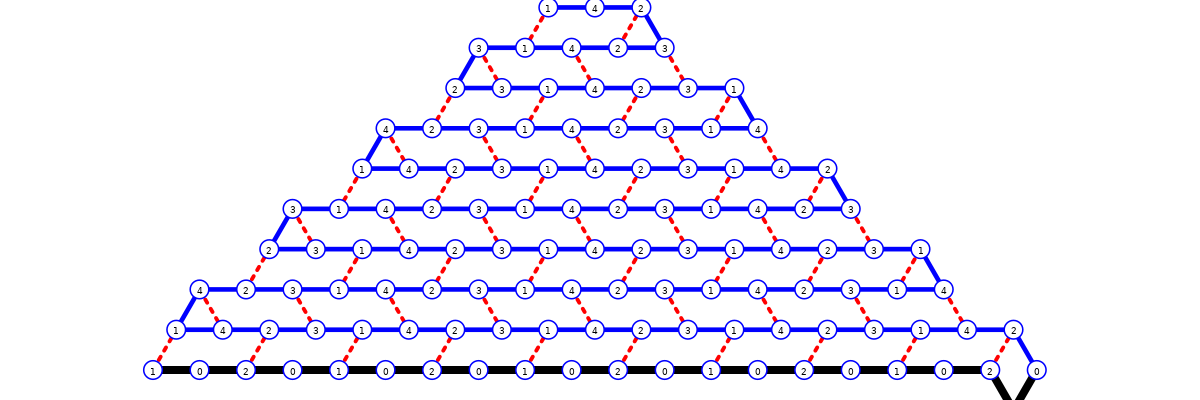
\includegraphics[width=0.9\linewidth]{./Fig/CI_Numbers}
	\caption{Quadratic length transcript folding deterministically into pyramid shape. Seed: thick black path. Transcript: thin blue path. Bonds: dashed red lines. }
	\label{CI:big}
\end{figure}


Stabilizing the first bead of row $j$ goes as follows (see Fig.~\ref{CI:turn}):
%\begin{itemize}
%	\item $\bf j\equiv 1\mod 4$: the first two beads are $24$, and the preceding bead is stabilized at $(4k-\frac{j-1}{2}, j-1)$. The $2$ can only bind to the $2$ which occurred two beads before at $(4k-\frac{j+1}{2}, j-1)$, and $4$ cannot bind anywhere, so the $2$ is stabilized at $(4k-\frac{j-1}{2},j)$.
%\end{itemize}

\begin{center}
	\begin{tabular}{|c|c|c|c|c|@{}m{0pt}@{}}
		%\renewcommand{\arraystretch}{2}
	$j\mod 4$					& first bead 	& predecessor at		& first bead binds to		& first stabilizes at\\
						\hline
	$\equiv 1$	& 2		& $(4k-\frac{j-1}{2}, j-1)$		& $(4k-\frac{j+1}{2}, j-1)$	& $(4k-\frac{j+1}{2}, j)$& $\mathrm{ }$\newline $\mathrm{ }$\\
	\hline
	$\equiv 2$	& 4				& $(\frac{3j}{2}-1,j-1)$		& $(\frac{3j}{2},j-1)$		& $(\frac{3j}{2},j)$ & $\mathrm{ }$\newline $\mathrm{ }$\\
	\hline
	$\equiv 3$	& 1				& $(4k-\frac{j-1}{2}, j-1)$		& $(4k-\frac{j+1}{2}, j-1)$	& $(4k-\frac{j+1}{2}, j)$ & $\mathrm{ }$\newline $\mathrm{ }$ \\
	\hline
	$\equiv 4$	& 3				& $(\frac{3j}{2}-1,j-1)$		& $(\frac{3j}{2},j-1)$		& $(\frac{3j}{2},j)$ & $\mathrm{ }$\newline $\mathrm{ }$ \\
	\hline		
	\end{tabular}
\end{center}



%The first bead of the transcript is type $2$ and it has to be fixed next to $(4k,0)$. The second bead is type $4$, which cannot form a bond with anything in the conformation so far. The only possibility of forming a bond is if the $2$-bead is placed at $(4k,1)$ and it bonds with the $2$-bead of the seed at $(4k-1,0)$. The next to be stabilized is a $4$-bead, and since it cannot form any bond, the conformation with the highest number of bonds is when the one after, a $1$-bead, is at $(4k-2,1)$ bonding with $(4k-3,0)$, which stabilizes the preceding $4$-bead at $(4k-1,1)$ (see Fig.~\ref{CI:1-4}, (a)-(b)).



\begin{figure}
	\begin{minipage}{.35\textwidth}
		\centering
		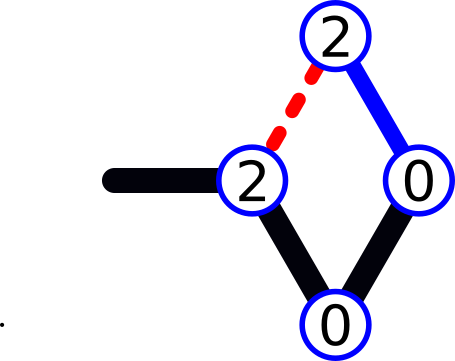
\includegraphics[align=c,height=1in]{./Fig/CI_1n}\\
		\bigskip
		
		(a) First transcript bead
	\end{minipage}%
	\begin{minipage}{.2\textwidth}
		\centering
		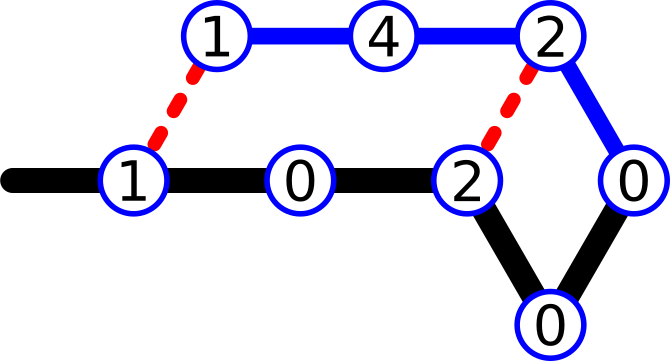
\includegraphics[align=c,height=0.7in]{./Fig/CI_2n}\\
		\bigskip
		
		(b) Second bead
	\end{minipage}
	\begin{minipage}{.4\textwidth}
		\centering
		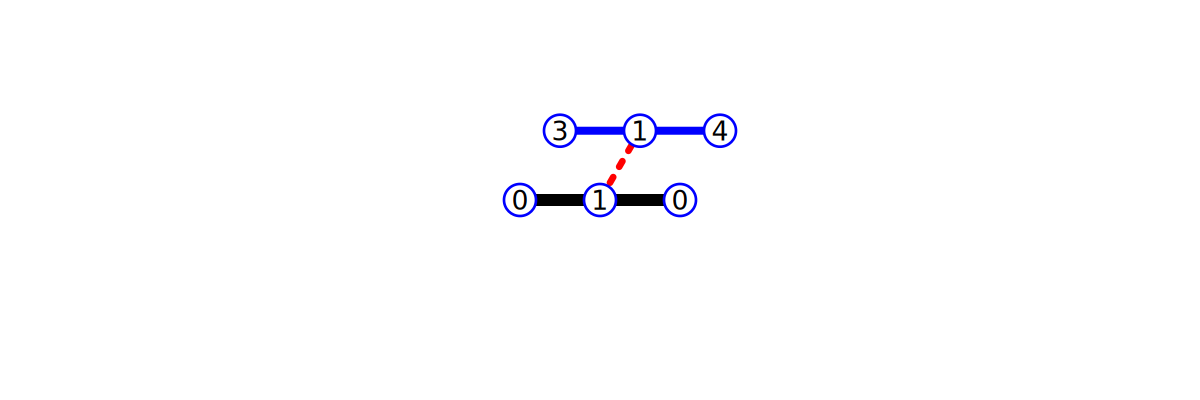
\includegraphics[align=c,height=0.5in]{./Fig/CI_3n}
		\bigskip
		\vspace{0.1in}
		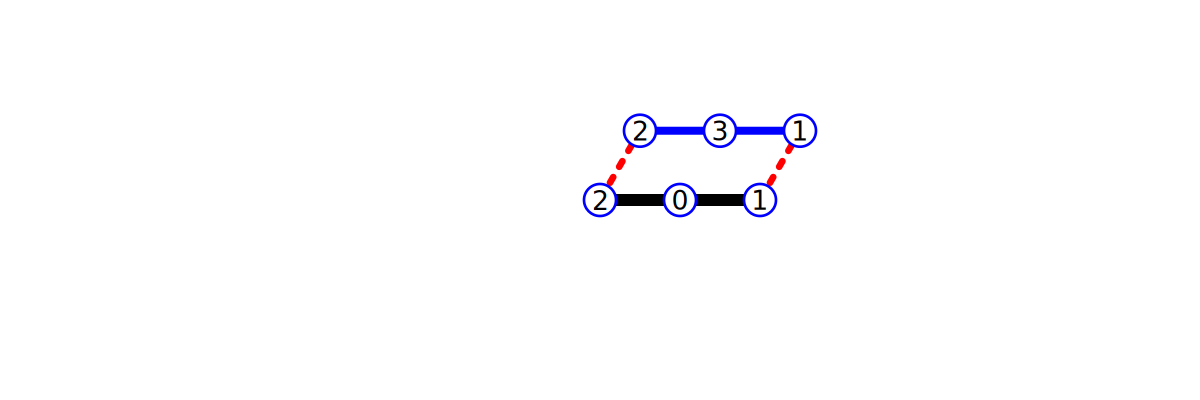
\includegraphics[align=c,height=0.5in]{./Fig/CI_4n}
		\bigskip
		
		(c) Portions of row $1$
	\end{minipage}
	\caption{Fixing transcript beads in odd rows}
	\label{CI:1-4}
\end{figure}


As for the other beads, in rows $j\equiv 1,3\mod 4$, beads of type $1$ and $3$ bind to a bead in row $j-1$. In rows $j\equiv 2,4\mod 4$ beads of type $2$ and $4$ can bind to a bead in row $j-1$.  This is true for row $1$, because beads of type $1$ and $3$ from row $1$ can only bind to every second bead of the seed, whereas beads of type $2$ and $4$ from row $1$ cannot bind to anything (Fig.~\ref{CI:1-4}, (c)). Once this dynamic holds for a row, it holds inductively for the next, as a bead that binds to another loses its only free hand at arity $1$.

Within one row of the transcript, no bead can bind to a preceding bead, because if there is a previous bead of the same type in that row, it is stabilized at a distance of four and the system has delay $2$.

By the arguments above, the beads in row $i$ of the transcript are stabilized along row $i$ on the grid, forming the pyramid-like conformation from Fig.~\ref{CI:big}.


\begin{figure}
	\centering
	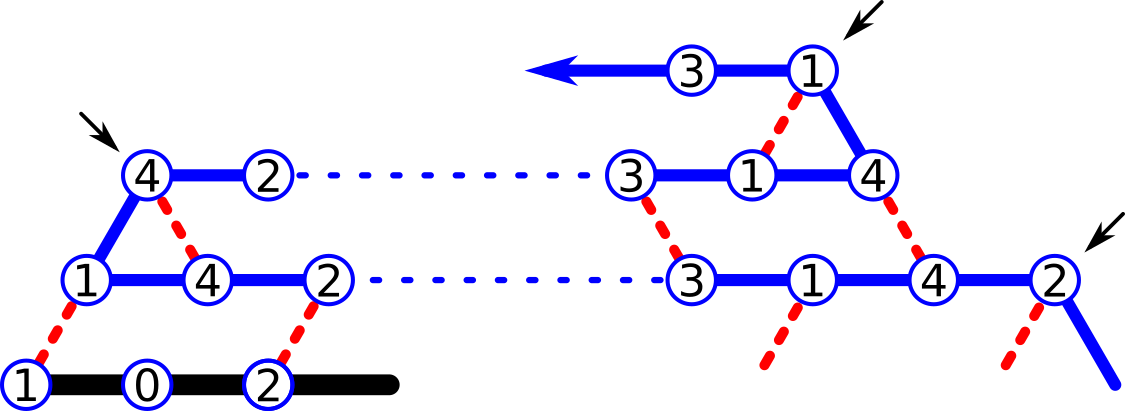
\includegraphics[width=0.7\linewidth]{./Fig/CI_turnn}
	\caption{Beads $4k, 8k-2, \dots$ stabilize at turning points because the bead two positions before is the same type and has a free hand.}
	\label{CI:turn}
\end{figure}




\subsection{$\alpha = 1$, unary}
\label{sec:unary}

Let the point where the first transcript bead was fixed be $p$ and let $n=|\mathrm{seed}|+1$. We will argue about the situation when the first bead is stabilized outside $\hexagon_p^n$ (a hexagon of radius $n$). Let this be the $i$th bead of the transcript. Without loss of generality, we can translate the origin $(0,0)$ to the coordinates of bead $i-1$ (which is still in $\hexagon_p^n$), and we can assume that the bead outside the hexagon is fixed at $(1,1)$ (see Fig.~\ref{fig:hexagonOut}).
\begin{figure}
	\centering
	\includegraphics[width=0.3\linewidth]{./Fig/hexagonOut}
	\caption{$\hexagon_p^n$ and the position $(1,1)$ of the first bead fixed outside of it.}
	\label{fig:hexagonOut}
\end{figure}

\subsubsection{\ref{sec:unary}.1 \ \ $\delta = 2$\\}

In the elongation that places bead $i$ at $(1,1)$ there are two possibilities:
\begin{itemize}
	\item $i$ forms a bond with a bead at $(1,0)$.
	\item  $i$ does not bond to anything and $i+1$ is at $(2,1)$ bonding with a bead at $(2,0)$. If there is no bead at $(1,0)$, then placing $i$ at $(1,0)$ instead of $(1,1)$ results in the same number of bonds, leading to nondeterminism. Therefore, there has to be a bead at $(1,0)$ and it is inactive, otherwise it would bond to $i$. This is analogous to case 1. below.%as in Fig.~\ref{fig:hexagonOut1}.
	\begin{figure}
		\centering
		\includegraphics[width=0.2\linewidth]{./Fig/hexagonOut1}
		%\caption{}
		\label{fig:hexagonOut1}
	\end{figure}
	
\end{itemize}
 
%The only position with which $(1,1)$ can form a bond is $(1,0)$. This means that there is a bead at $(1,0)$, which bonds to bead $i$, otherwise there are other conformations in which beads $i$ and $i+1$ add one bond to the conformation, making the behavior nondeterministic.

The next bead, $i+1$, can be fixed at $(2,1)$ or at $(0,1)$ as all other possibilities result in nondeterministic behavior immediately, so we have two cases.

\begin{enumerate}
	\item bead $i+1$ is fixed at $(2,1)$ and can bond with a bead at $(2,0)$. Now consider bead $i+2$. For $i+1$ to be fixed at $(2,1)$, $i+2$ needs to form a bond somewhere, otherwise $i+2$ could go to $(2,1)$ forming the bond with the bead at $(2,0)$ and there would be two conformations with the maximal $1$ bond. The only possibility is that there is a bead at $(3,0)$ and $i+2$ can bond with it when placed at $(3,1)$. We can apply the same argument inductively: there is some $m\geq 0$ such that grid points $(\ell,0)$ are occupied by active beads, for all $\ell\in \{2,\dots,2+m\}$, and there is no bead at $(3+m,0)$. Such an $m$ exists, and it is not greater than $n$. Then, bead $i+\ell$ is fixed at $(\ell+1,1)$ and bonds with $(\ell+1,0)$. However, bead $i+2+m$ cannot be fixed anywhere, because $i+2+m$ and $i+3+m$ can only add one bond to the conformation, and that is possible either with $i+2+m \rightarrow (2+m,1)$, $i+3+m \rightarrow (3+m,1)$ or with $i+2+m \rightarrow (2+m,2)$, $i+3+m \rightarrow (2+m,1)$. 
	\begin{figure}
		\centering
		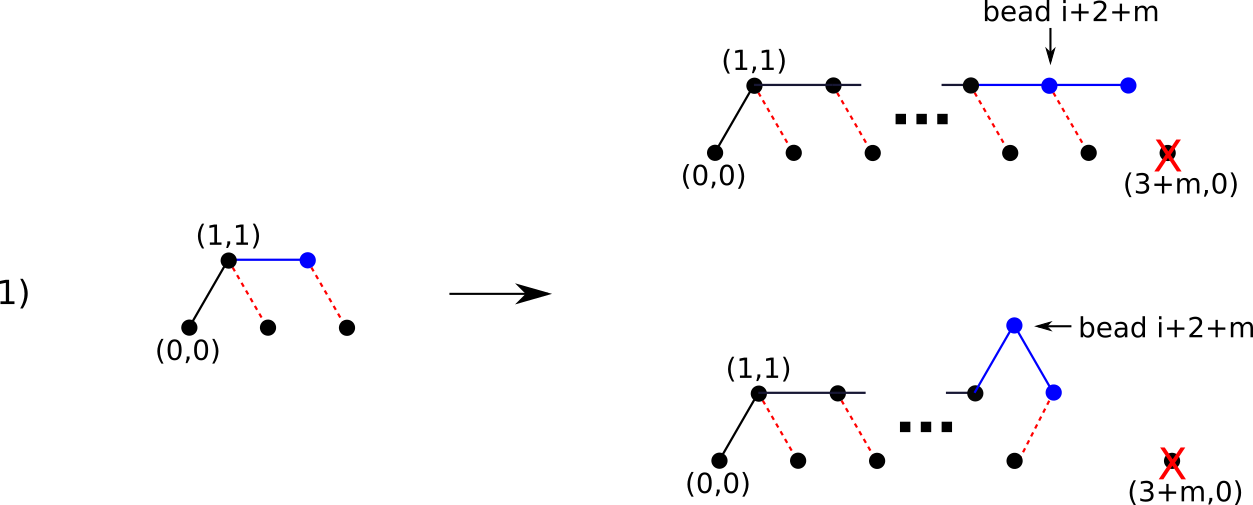
\includegraphics[width=0.9\linewidth]{./Fig/hexagonOut2}
		\caption{When bead $i+2+m$ is fixed}
		\label{fig:hexagonout2}
	\end{figure}
	
	\item bead $i+1$ is fixed at $(0,1)$. This is only possible if
	\begin{enumerate}
		\item there is an inactive bead at $(-1,0)$ and an active one at $(-2,0)$. This case is symmetrical to (1).
		\item there is no bead at $(-1,0)$, bead $i+1$ can bond with bead $i-1$ at $(0,0)$ and the bead $i+2$ can be placed at $(-1,0)$ where it can bond with $(-2,0)$, $(-2,-1)$ or $(-1,-1)$. This leads to nondeterminism, because bead $i$ at $(-1,0)$ and bead $i+1$ at $(0,1)$ has two bonds, just as the original conformation.
		\item there is a bead at $(-1,0)$ and bead $i+1$ can bond with that or with bead $i-1$ at $(0,0)$. However, this means that placing bead $i$ at $(0,1)$ at bead $i+1$ at $(1,1)$ creates the same number of hydrogen bonds, thus resulting in bead $i$ not being placed deterministically.
		
	\end{enumerate}
\end{enumerate}




\begin{figure}
	\centering
	%\includegraphics[width=0.3\linewidth]{./hexagonOut1}
	%\hspace{10mm} %
	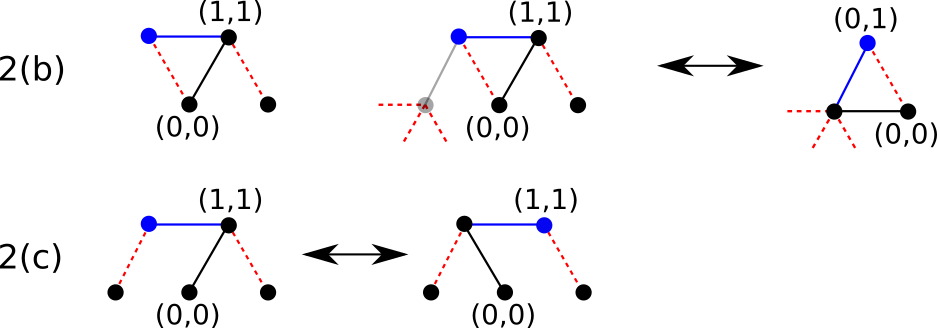
\includegraphics[width=0.8\linewidth]{./Fig/hexagonOut3n}
	
	\caption{When bead $i+1$ is fixed at (0,1)}
	\label{fig:hexagonOut2}
\end{figure}


\subsubsection{\ref{sec:unary}.2 \ \ $\delta = 3$\\}

\begin{enumerate}
\item Let us discuss that a fixed bead on a side of $\hexagon_p^n$ has a free hand, and bead $i$ binds to it. If the most stable conformation formed by beads $i, i+1, i+2$ has only two hydrogen bonds, it will be nondeterministic because there are at least two possibilities, see Fig.~\ref{fig:beadi}. Therefore, it needs to make three hydrogen bonds to deterministically stabilize $i$.\\

\begin{figure}
  \begin{center}
    \begin{tabular}{cc}
      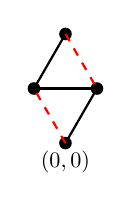
\begin{tikzpicture}[thick,scale=0.8, every node/.style={scale=0.8}]
        \fill (0.0, 0.0) circle [radius = 0.1];
        \fill (0.5, 0.866) circle [radius = 0.1];
        \fill (-0.5, 0.866) circle [radius = 0.1];
        \fill (0.0, 1.732) circle [radius = 0.1];
        \fill (0.0, 0.0) node [below] {$(0, 0)$};
        \draw (0.0, 0.0) -- (0.5, 0.866);
        \draw (0.5, 0.866) -- (-0.5, 0.866);
        \draw (0.0, 1.732) -- (-0.5, 0.866);
        \draw [dashed] [red] (0.0, 1.732) -- (0.5, 0.866);
        \draw [dashed] [red] (0.0, 0.0) -- (-0.5, 0.866);
      \end{tikzpicture}

      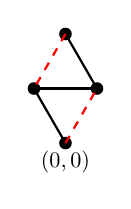
\begin{tikzpicture}[thick,scale=0.8, every node/.style={scale=0.8}]
        \fill (0.0, 0.0) circle [radius = 0.1];
        \fill (-0.5, 0.866) circle [radius = 0.1];
        \fill (0.5, 0.866) circle [radius = 0.1];
        \fill (0.0, 1.732) circle [radius = 0.1];
        \fill (0.0, 0.0) node [below] {$(0, 0)$};
        \draw (0.0, 0.0) -- (-0.5, 0.866);
        \draw (-0.5, 0.866) -- (0.5, 0.866);
        \draw (0.0, 1.732) -- (0.5, 0.866);
        \draw [dashed] [red] (0.0, 0.0) -- (0.5, 0.866);
        \draw [dashed] [red] (0.0, 1.732) -- (-0.5, 0.866);
      \end{tikzpicture}

    \end{tabular}
    \caption{Two conformations when bead $i-1$ at (0,0) has a free hand}
    \label{fig:beadi}
  \end{center}
\end{figure}



\begin{figure}
  \begin{center}
    \begin{tabular}{ccccc}
      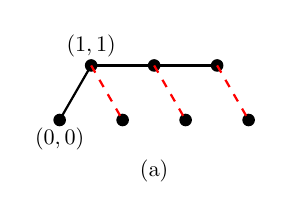
\begin{tikzpicture}[thick,scale=0.8, every node/.style={scale=0.8}]
        \fill (0.0, 0.0) circle [radius = 0.1];
        \fill (1.0, 0.0) circle [radius = 0.1];
        \fill (2.0, 0.0) circle [radius = 0.1];
        \fill (3.0, 0.0) circle [radius = 0.1];
        \fill (0.5, 0.866) circle [radius = 0.1];
        \fill (1.5, 0.866) circle [radius = 0.1];
        \fill (2.5, 0.866) circle [radius = 0.1];
        \fill (0.0, 0.0) node [below] {$(0, 0)$};
        \fill (0.5, 0.866) node [above] {$(1, 1)$};
        \draw (0.0, 0.0) -- (0.5, 0.866);
        \draw (0.5, 0.866) -- (1.5, 0.866);
        \draw (1.5, 0.866) -- (2.5, 0.866);
        \draw [dashed] [red] (0.5, 0.866) -- (1.0, 0.0);
        \draw [dashed] [red] (1.5, 0.866) -- (2.0, 0.0);
        \draw [dashed] [red] (2.5, 0.866) -- (3.0, 0.0);
        \fill (1.5, -0.5) node [below] {(a)};
      \end{tikzpicture}

      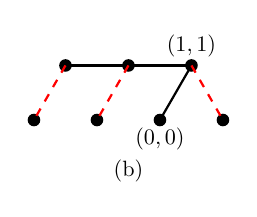
\begin{tikzpicture}[thick,scale=0.8, every node/.style={scale=0.8}]
        \fill (1.0, 0.0) circle [radius = 0.1];
        \fill (0.0, 0.0) circle [radius = 0.1];
        \fill (-1.0, 0.0) circle [radius = 0.1];
        \fill (-2.0, 0.0) circle [radius = 0.1];
        \fill (0.5, 0.866) circle [radius = 0.1];
        \fill (-0.5, 0.866) circle [radius = 0.1];
        \fill (-1.5, 0.866) circle [radius = 0.1];
        \fill (0.0, 0.0) node [below] {$(0, 0)$};
        \fill (0.5, 0.866) node [above] {$(1, 1)$};
        \draw (0.0, 0.0) -- (0.5, 0.866);
        \draw (0.5, 0.866) -- (-0.5, 0.866);
        \draw (-0.5, 0.866) -- (-1.5, 0.866);
        \draw [dashed] [red] (0.5, 0.866) -- (1.0, 0.0);
        \draw [dashed] [red] (-0.5, 0.866) -- (-1.0, 0.0);
        \draw [dashed] [red] (-1.5, 0.866) -- (-2.0, 0.0);
        \fill (-0.5, -0.5) node [below] {(b)};
      \end{tikzpicture}

      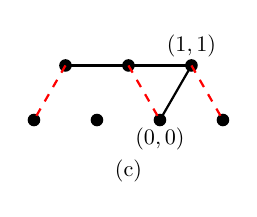
\begin{tikzpicture}[thick,scale=0.8, every node/.style={scale=0.8}]
        \fill (1.0, 0.0) circle [radius = 0.1];
        \fill (0.0, 0.0) circle [radius = 0.1];
        \fill (-1.0, 0.0) circle [radius = 0.1];
        \fill (-2.0, 0.0) circle [radius = 0.1];
        \fill (0.5, 0.866) circle [radius = 0.1];
        \fill (-0.5, 0.866) circle [radius = 0.1];
        \fill (-1.5, 0.866) circle [radius = 0.1];
        \fill (0.0, 0.0) node [below] {$(0, 0)$};
        \fill (0.5, 0.866) node [above] {$(1, 1)$};
        \draw (0.0, 0.0) -- (0.5, 0.866);
        \draw (0.5, 0.866) -- (-0.5, 0.866);
        \draw (-0.5, 0.866) -- (-1.5, 0.866);
        \draw [dashed] [red] (0.5, 0.866) -- (1.0, 0.0);
        \draw [dashed] [red] (-0.5, 0.866) -- (0.0, 0.0);
        \draw [dashed] [red] (-1.5, 0.866) -- (-2.0, 0.0);
        \fill (-0.5, -0.5) node [below] {(c)};
      \end{tikzpicture}

      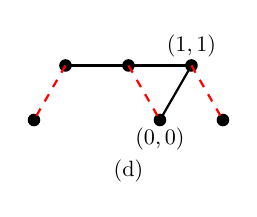
\begin{tikzpicture}[thick,scale=0.8, every node/.style={scale=0.8}]
        \fill (1.0, 0.0) circle [radius = 0.1];
        \fill (0.0, 0.0) circle [radius = 0.1];
        \fill (-2.0, 0.0) circle [radius = 0.1];
        \fill (0.5, 0.866) circle [radius = 0.1];
        \fill (-0.5, 0.866) circle [radius = 0.1];
        \fill (-1.5, 0.866) circle [radius = 0.1];
        \fill (0.0, 0.0) node [below] {$(0, 0)$};
        \fill (0.5, 0.866) node [above] {$(1, 1)$};
        \draw (0.0, 0.0) -- (0.5, 0.866);
        \draw (0.5, 0.866) -- (-0.5, 0.866);
        \draw (-0.5, 0.866) -- (-1.5, 0.866);
        \draw [dashed] [red] (0.5, 0.866) -- (1.0, 0.0);
        \draw [dashed] [red] (-0.5, 0.866) -- (0.0, 0.0);
        \draw [dashed] [red] (-1.5, 0.866) -- (-2.0, 0.0);
        \fill (-0.5, -0.5) node [below] {(d)};
      \end{tikzpicture}

      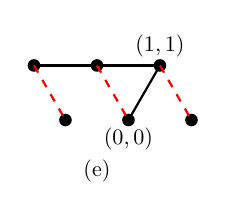
\begin{tikzpicture}[thick,scale=0.8, every node/.style={scale=0.8}]
        \fill (1.0, 0.0) circle [radius = 0.1];
        \fill (0.0, 0.0) circle [radius = 0.1];
        \fill (-1.0, 0.0) circle [radius = 0.1];
        \fill (0.5, 0.866) circle [radius = 0.1];
        \fill (-0.5, 0.866) circle [radius = 0.1];
        \fill (-1.5, 0.866) circle [radius = 0.1];
        \fill (0.0, 0.0) node [below] {$(0, 0)$};
        \fill (0.5, 0.866) node [above] {$(1, 1)$};
        \draw (0.0, 0.0) -- (0.5, 0.866);
        \draw (0.5, 0.866) -- (-0.5, 0.866);
        \draw (-0.5, 0.866) -- (-1.5, 0.866);
        \draw [dashed] [red] (0.5, 0.866) -- (1.0, 0.0);
        \draw [dashed] [red] (-0.5, 0.866) -- (0.0, 0.0);
        \draw [dashed] [red] (-1.5, 0.866) -- (-1.0, 0.0);
        \fill (-0.5, -0.5) node [below] {(e)};
      \end{tikzpicture}\\

    \end{tabular}
    \caption{When beads $i, i+1, i+2$ make three hydrogen bonds \newline (c) there is an inactive bead at (-1,0). \newline (d) there is no bead at (-1,0).}
    \label{fig:3bonds}
  \end{center}
\end{figure}

There are the five cases in which beads $i, i+1, i+2$ can have three bonds, see Fig.~\ref{fig:3bonds}. There are beads having a free hand at (1,0) and (-1,0) to realize (b) and (e) in Fig.~\ref{fig:3bonds} before a bead $i-1$ is fixed at (0,0). One of these two beads may be a predecessor of a bead $i-1$, but at least one bead is not. A bead $i-1$ makes a hydrogen bond with one of these two beads which is not its predecessor when it is fixed at (0,0). That is, it is impossible to put three beads having a free hand at (-1,0), (0,0) and (1,0) when a bead $i$ is fixed, and then, to realize (b) and (e) in Fig.~\ref{fig:3bonds}. (d) in Fig.~\ref{fig:3bonds} becomes nondeterministic when bead $i$ is fixed because bead $i$ can be fixed at (-1,0) and bond with (-2,0), bead $i+1$ can be placed (0,1) and bond with (0,0) and bead $i+2$ can be placed (1,1) and bond with (0,1). If it makes three bonds once, such as (a) and (c) in Fig.~\ref{fig:3bonds}, it will need to make three bonds forever to be deterministic. Similarly to case 1. in the previous section, (a) and (c) in Fig.~\ref{fig:3bonds} become nondeterministic finally when it reaches a first corner of $\hexagon_p^n$.



\item Let us discuss that bead $i$'s predecessor at (0,0) has no free hand. Let us assume that there is a bead at (1,0) which has a free hand. If there is a bead at (1,0) and beads $i, i+1, i+2$ make only two hydrogen bonds, it will become nondeterministic as in Fig.~\ref{fig:beadat(1,0)}. That is, beads $i, i+1, i+2$ need to make three bonds to stabilize $i$. If they make three hydrogen bonds, the situation is analogous to (a) and (c) in Fig.~\ref{fig:3bonds}. There are not any bead having a free hand at (1,0) or (-1,0) to prevent from being (a) and (c) in Fig.~\ref{fig:3bonds}. Let us discuss the moment after bead $i$ is fixed outside $\hexagon_p^n$. Now bead $i$ has a free hand because there are no beads having a free hand at (1,0) or (-1,0). If beads $i+1, i+2, i+3$ can form only two bonds, it will be nondeterministic because there are at least two possible such conformations, as in Fig.~\ref{fig:beadi2}. Hence, they need to form three bonds to deterministically stabilize, such as in Fig.~\ref{fig:3bonds2}. (a) in Fig~\ref{fig:3bonds2} becomes (a) in Fig.~\ref{fig:3bonds}. (b) in Fig.~\ref{fig:3bonds2} becomes nondeterministic when bead $i$ is fixed because bead $i$ can be fixed at (1,0).\\

\begin{figure}
  \begin{center}
    \begin{tabular}{cc}
      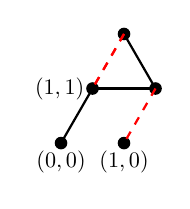
\begin{tikzpicture}[thick,scale=0.8, every node/.style={scale=0.8}]
        \fill (0.0, 0.0) circle [radius = 0.1];
        \fill (1.0, 0.0) circle [radius = 0.1];
        \fill (0.5, 0.866) circle [radius = 0.1];
        \fill (1.5, 0.866) circle [radius = 0.1];
        \fill (1.0, 1.732) circle [radius = 0.1];
        \fill (0.0, 0.0) node [below] {$(0, 0)$};
        \fill (0.5, 0.866) node [left] {$(1, 1)$};
        \fill (1.0, 0.0) node [below] {$(1, 0)$};
        \draw (0.0, 0.0) -- (0.5, 0.866);
        \draw (0.5, 0.866) -- (1.5, 0.866);
        \draw (1.0, 1.732) -- (1.5, 0.866);
        \draw [dashed] [red] (1.5, 0.866) -- (1.0, 0.0);
        \draw [dashed] [red] (1.0, 1.732) -- (0.5, 0.866);
        \draw [dashed] [red] (1.0, 1.732) -- (0.5, 0.866);
      \end{tikzpicture}

      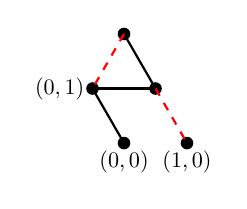
\begin{tikzpicture}[thick,scale=0.8, every node/.style={scale=0.8}]
        \fill (0.0, 0.0) circle [radius = 0.1];
        \fill (1.0, 0.0) circle [radius = 0.1];
        \fill (-0.5, 0.866) circle [radius = 0.1];
        \fill (0.5, 0.866) circle [radius = 0.1];
        \fill (0.0, 1.732) circle [radius = 0.1];
        \fill (0.0, 0.0) node [below] {$(0, 0)$};
        \fill (-0.5, 0.866) node [left] {$(0, 1)$};
        \fill (1.0, 0.0) node [below] {$(1, 0)$};
        \draw (0.0, 0.0) -- (-0.5, 0.866);
        \draw (-0.5, 0.866) -- (0.5, 0.866);
        \draw (0.0, 1.732) -- (0.5, 0.866);
        \draw [dashed] [red] (0.5, 0.866) -- (1.0, 0.0);
        \draw [dashed] [red] (0.0, 1.732) -- (-0.5, 0.866);
      \end{tikzpicture}

    \end{tabular}
    \caption{Two conformations when a bead at (1,0) has a free hand}
    \label{fig:beadat(1,0)}
  \end{center}
\end{figure}



\begin{figure}
  \begin{center}
    \begin{tabular}{cc}
      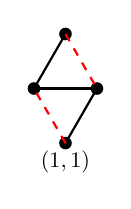
\begin{tikzpicture}[thick,scale=0.8, every node/.style={scale=0.8}]
        \fill (0.0, 0.0) circle [radius = 0.1];
        \fill (0.5, 0.866) circle [radius = 0.1];
        \fill (-0.5, 0.866) circle [radius = 0.1];
        \fill (0.0, 1.732) circle [radius = 0.1];
        \fill (0.0, 0.0) node [below] {$(1, 1)$};
        \draw (0.0, 0.0) -- (0.5, 0.866);
        \draw (0.5, 0.866) -- (-0.5, 0.866);
        \draw (0.0, 1.732) -- (-0.5, 0.866);
        \draw [dashed] [red] (0.0, 1.732) -- (0.5, 0.866);
        \draw [dashed] [red] (0.0, 0.0) -- (-0.5, 0.866);
      \end{tikzpicture}

      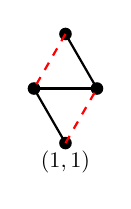
\begin{tikzpicture}[thick,scale=0.8, every node/.style={scale=0.8}]
        \fill (0.0, 0.0) circle [radius = 0.1];
        \fill (-0.5, 0.866) circle [radius = 0.1];
        \fill (0.5, 0.866) circle [radius = 0.1];
        \fill (0.0, 1.732) circle [radius = 0.1];
        \fill (0.0, 0.0) node [below] {$(1, 1)$};
        \draw (0.0, 0.0) -- (-0.5, 0.866);
        \draw (-0.5, 0.866) -- (0.5, 0.866);
        \draw (0.0, 1.732) -- (0.5, 0.866);
        \draw [dashed] [red] (0.0, 0.0) -- (0.5, 0.866);
        \draw [dashed] [red] (0.0, 1.732) -- (-0.5, 0.866);
      \end{tikzpicture}

    \end{tabular}
    \caption{Two conformations when a bead $i$ at (1,1) has a free hand}
    \label{fig:beadi2}
  \end{center}
\end{figure}



\begin{figure}
  \begin{center}
    \begin{tabular}{cc}

      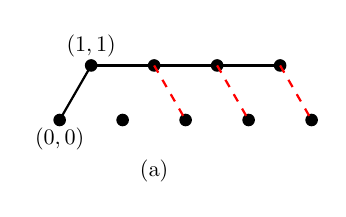
\begin{tikzpicture}[thick,scale=0.8, every node/.style={scale=0.8}]
        \fill (0.0, 0.0) circle [radius = 0.1];
        \fill (1.0, 0.0) circle [radius = 0.1];
        \fill (2.0, 0.0) circle [radius = 0.1];
        \fill (3.0, 0.0) circle [radius = 0.1];
        \fill (4.0, 0.0) circle [radius = 0.1];
        \fill (0.5, 0.866) circle [radius = 0.1];
        \fill (1.5, 0.866) circle [radius = 0.1];
        \fill (2.5, 0.866) circle [radius = 0.1];
        \fill (3.5, 0.866) circle [radius = 0.1];
        \fill (0.0, 0.0) node [below] {$(0, 0)$};
        \fill (0.5, 0.866) node [above] {$(1, 1)$};
        \draw (0.0, 0.0) -- (0.5, 0.866);
        \draw (0.5, 0.866) -- (1.5, 0.866);
        \draw (1.5, 0.866) -- (2.5, 0.866);
        \draw (2.5, 0.866) -- (3.5, 0.866);
        \draw [dashed] [red] (1.5, 0.866) -- (2.0, 0.0);
        \draw [dashed] [red] (2.5, 0.866) -- (3.0, 0.0);
        \draw [dashed] [red] (3.5, 0.866) -- (4.0, 0.0);
        \fill (1.5, -0.5) node [below] {(a)};
      \end{tikzpicture}
      
      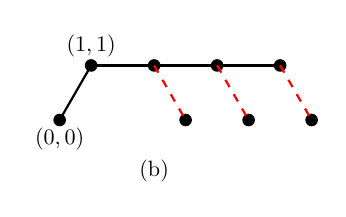
\begin{tikzpicture}[thick,scale=0.8, every node/.style={scale=0.8}]
        \fill (0.0, 0.0) circle [radius = 0.1];
        \fill (2.0, 0.0) circle [radius = 0.1];
        \fill (3.0, 0.0) circle [radius = 0.1];
        \fill (4.0, 0.0) circle [radius = 0.1];
        \fill (0.5, 0.866) circle [radius = 0.1];
        \fill (1.5, 0.866) circle [radius = 0.1];
        \fill (2.5, 0.866) circle [radius = 0.1];
        \fill (3.5, 0.866) circle [radius = 0.1];
        \fill (0.0, 0.0) node [below] {$(0, 0)$};
        \fill (0.5, 0.866) node [above] {$(1, 1)$};
        \draw (0.0, 0.0) -- (0.5, 0.866);
        \draw (0.5, 0.866) -- (1.5, 0.866);
        \draw (1.5, 0.866) -- (2.5, 0.866);
        \draw (2.5, 0.866) -- (3.5, 0.866);
        \draw [dashed] [red] (1.5, 0.866) -- (2.0, 0.0);
        \draw [dashed] [red] (2.5, 0.866) -- (3.0, 0.0);
        \draw [dashed] [red] (3.5, 0.866) -- (4.0, 0.0);
        \fill (1.5, -0.5) node [below] {(b)};
      \end{tikzpicture}\\

    \end{tabular}
    \caption{When beads $i+1, i+2, i+3$ make three hydrogen bonds \newline (a) there is an inactive bead at (1,0). \newline (b) there is no bead at (1,0).}
    \label{fig:3bonds2}
  \end{center}
\end{figure}

\end{enumerate}

It can yield only finite conformation and the length is $3n^2+n^2+1$.
